%%% Local Variables:
%%% mode: latex
%%% TeX-master: t
%%% End:

\section{The Necessity of Blockchain}

\subsection{What is Blockchain}

A blockchain is a growing list of records, called blocks, that are securely linked together using cryptography. Each block contains a cryptographic hash of the previous block, a timestamp, and transaction data (generally represented as a Merkle tree, where data nodes are represented by leafs). The timestamp proves that the transaction data existed when the block was published to get into its hash. As blocks each contain information about the block previous to it, they form a chain, with each additional block reinforcing the ones before it. Therefore, blockchains are resistant to modification of their data because once recorded, the data in any given block cannot be altered retroactively without altering all subsequent blocks. \\[-8pt]

Blockchains are typically managed by a peer-to-peer network for use as a publicly distributed ledger, where nodes collectively adhere to a protocol to communicate and validate new blocks. Although blockchain records are not unalterable as forks are possible, blockchains may be considered secure by design and exemplify a distributed computing system with high Byzantine fault tolerance.

\namedfigure
{!hbtp}
{img:bitcoinBlockchain}
{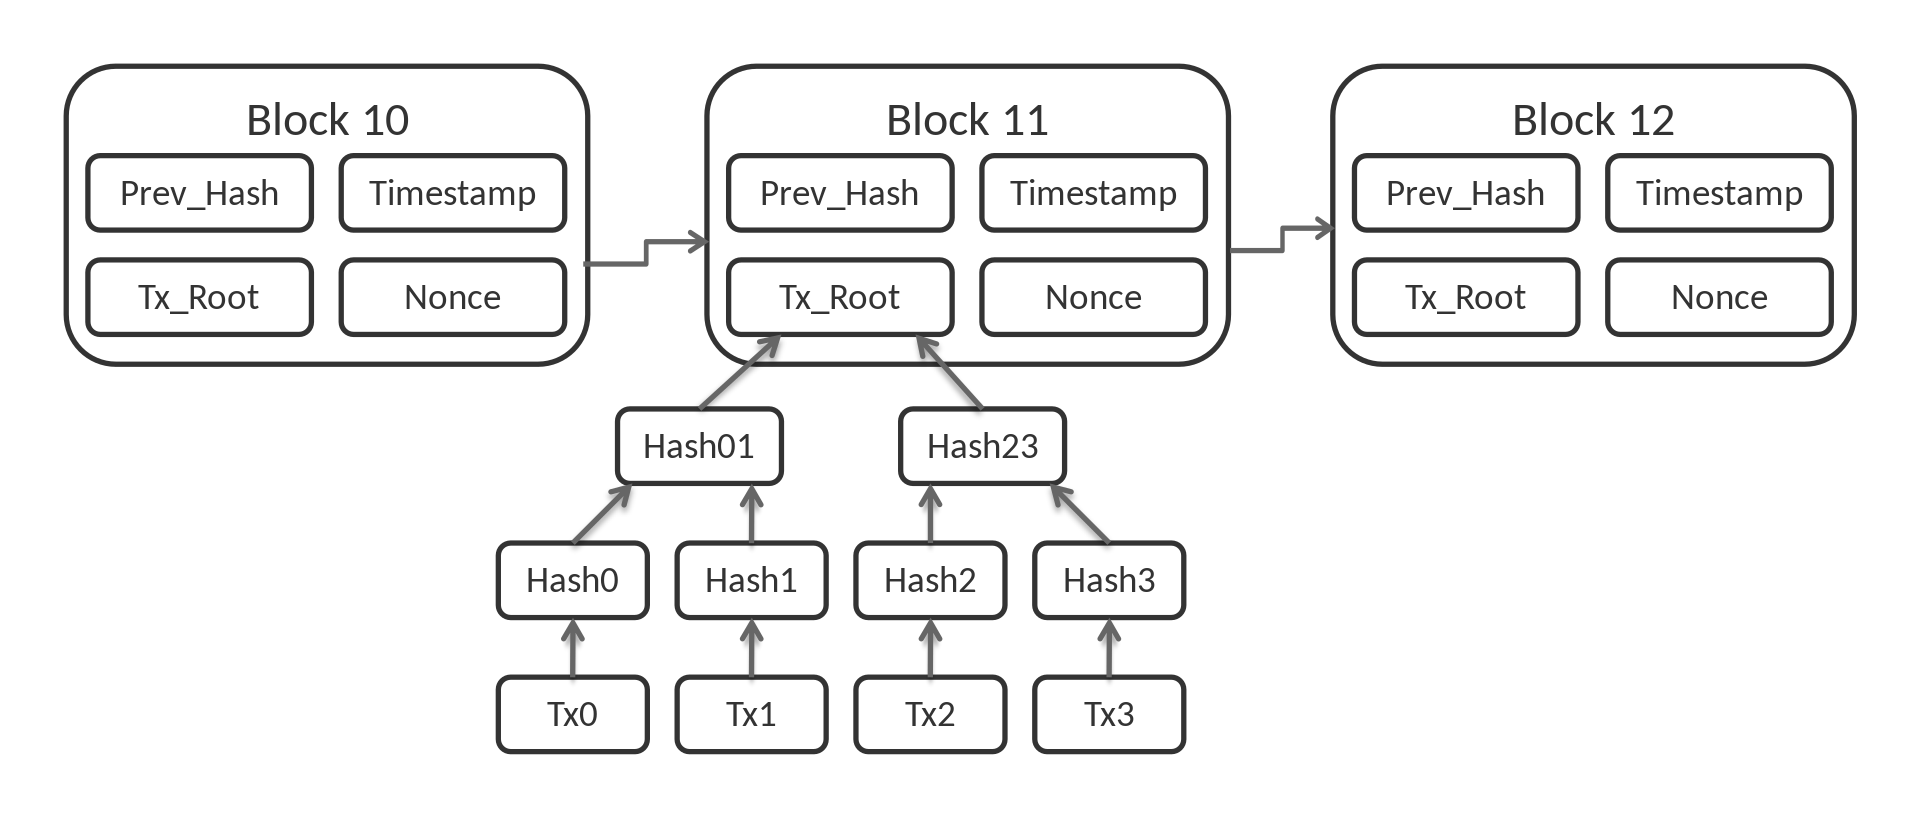
\includegraphics[width=\textwidth]{bitcoin_blockchain_structure.png}}
{Bitcoin blockchain structure.}


\subsection{Blockchain in The Cloud Storage Use Case}

For the system to be completely decentralized, we do not use centralized databases owned by a single entity, but we use Blockchain to keep track of users' files' metadata. \\[-8pt]

The immutable nature of blockchain, and the fact that every computer on the network is continually verifying the information stored on it, makes blockchain an excellent tool for storing data. \\[-8pt]

The blockchain will help reduce the security and data loss concerns associated with a typical public storage solution. Also, it will help reduce downtime on the cloud. Users with excess storage will have the option of renting out their spaces for a fee. \\[-8pt]

\noindent
There are many advantages to using blockchain technology compared to other traditional technologies listed below. \\

\begin{itemize}
\item \textbf{Transparency: } Blockchain makes transaction histories more transparent than they ever were. Because it is a type of a distributed ledger, all nodes in the network share a copy of the documentation.  The data on a blockchain ledger is easily accessible for everyone to view. If a transaction history changes, everyone in the network can see the change and the updated record. Therefore, all information about currency exchange is available to everyone. \\
\item \textbf{Security: } Blockchain is better than any other record-keeping system when it comes to security, by all standards. The shared documentation of transactions can only be updated and/or modified with consensus on a blockchain network. Only if everyone or a majority of nodes agree to update a record, the information is edited. Moreover, when a transaction is approved, it is encrypted and connected with the previous transaction. Therefore, no one person or party has the potential to alter a record.\\
\item \textbf{Traceability: } In complex supply chains, it is hard to trace products back to their origins. But, with blockchain, the exchanges of goods are recorded, so you get an audit trail to learn where a particular asset came from.\\
\item \textbf{Cost reduction: } As blockchain eliminates the need for third-parties and middlemen, it saves enormous costs for businesses. Given that you can trust the trading partner, you don’t need anyone else to establish the rules and policies of exchange.\\
\end{itemize}
